\documentclass[12pt, twoside]{article}
\usepackage[utf8]{inputenc}
\usepackage[english,russian]{babel}
\newcommand{\hdir}{.}

\usepackage{graphicx}
\usepackage{caption}
\usepackage{amssymb}
\usepackage{amsmath}
\usepackage{mathrsfs}
\usepackage{euscript}
\usepackage{upgreek}
\usepackage{array}
\usepackage{theorem}
\usepackage{graphicx}
\usepackage{subfig}
\usepackage{caption}
\usepackage{color}
\usepackage{url}

\usepackage{verbatim}

\usepackage[left=2cm,right=2cm,top=3cm,bottom=2cm,bindingoffset=0cm]{geometry}

\usepackage{fancyhdr}
\pagestyle{fancy}
\fancyhead{}
\fancyhead[LE,RO]{\thepage} 
\fancyhead[CO,CE]{Final Test}
\fancyhead[LO,LE]{Ф.И.О.}

\begin{document} 

\paragraph{1.} Опишите процесc компиляции программы.

\paragraph{2.} Определения: $f\left(n\right) \in O\left(g\left(n\right)\right)$, $f\left(n\right) \in \Omega\left(g\left(n\right)\right)$, $f\left(n\right) \in o\left(g\left(n\right)\right)$

\paragraph{3.} Упорядочите, что во что вложено в определении $O$-ассимптотике:
$$n; \log n; n^2; n^{\frac{3}{2}}; n^n; 10; 2^n; n!.$$

\paragraph{4.} Найдите ассимптотику по времени исполнения, а также укажите количество выделенной памяти в зависимости от длины входной строки для следующего кода:

\begin{verbatim}
#include <iostream>
#include <string.h>

const char number = 0xFFFF;

int function(const char* str){
    printf("%s\n", str);
    if(strlen(str) > 0){
        function(str+1);
    }
    return 0;
}

int main(){
    char a[number];
    // вводиться строка длины n
    scanf("%s", a);
    function(a);
    return 0;
}
\end{verbatim}

\paragraph{5.} Какие основные элементы классов?

\paragraph{6.} Укажите все известные вам структуры данных.

\begin{table}[h!]
\begin{center}
\caption{}
\label{table1}
\begin{tabular}{|c|c|c|c|}
\hline
Структура	&insert(index)	&pop(index)	&find(index)\\
\hline
List			&			&			&\\
\hline
Array		&			&			&\\
\hline
\end{tabular}
\end{center}
\end{table}

\paragraph{7.} Что такое стек, очередь? В чем отличие?

\paragraph{8.} Заполните таблицу~\ref{table1} асимптотическим временем выполнения операций в терминах $O\left(n\right),$ где $n$ --- это количество элементов в структуре данных. 

\paragraph{9.} Опишите алгоритм, для нахождения минимального пути в таблице~\ref{table2} из правой верхней клетки в нижнюю левую клетку, если можно итти только влево или вниз.

\begin{table}[h!]
\begin{center}
\caption{}
\label{table2}
\begin{tabular}{|c|c|c|c|c|c|c|}
\hline
0	&7	&2	&5	&9	&2	&7\\
\hline
4	&6	&6	&6	&4	&3	&8\\
\hline
3	&6	&4	&4	&3	&8	&7\\
\hline
3	&2	&7	&2	&2	&7	&9\\
\hline
4	&5	&8	&2	&6	&5	&6\\
\hline
\end{tabular}
\end{center}
\end{table}


\paragraph{10.} Определение графа и дерева.

\paragraph{11.} Продемонстрируйте обход графа при помощи поиска в ширину для графа на рис.~\ref{fig1}. Начальные вершины выбираете на свое усмотрение.


\begin{figure}[h!t]\center
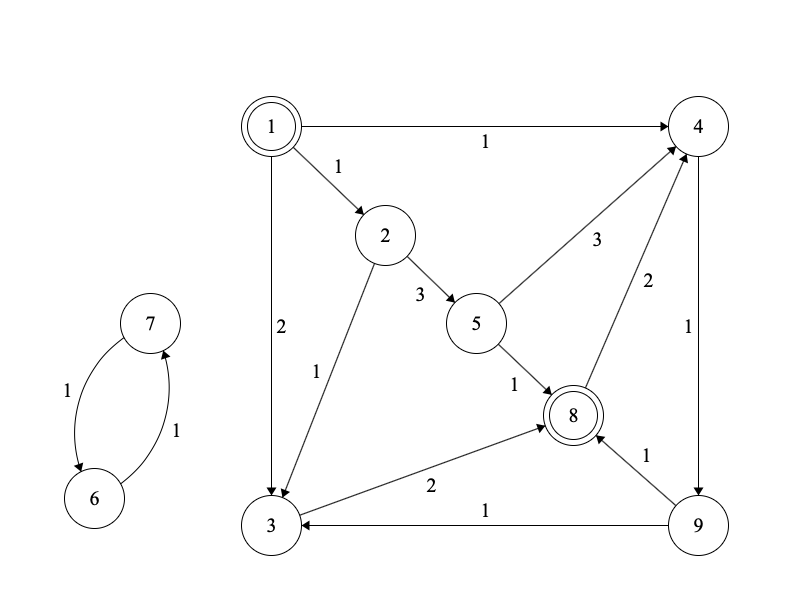
\includegraphics[width=0.5\textwidth]{1}
\caption{}
\label{fig1}
\end{figure}

\paragraph{12.} Продемонстрируйте обход графа при помощи поиска в глубину для графа на рис.~\ref{fig1}. Начальные вершины выбираете на свое усмотрение.

\paragraph{13.} Продемонстрируйте обход графа при помощи поиска в глубину для графа на рис.~\ref{fig1}. Начальные вершины выбираете на свое усмотрение.


\paragraph{14.} Продемонстрируйте работу алгоритма Дейкстры для графа на рис.~\ref{fig1}. Начальная вершина $1$. Укажите расстояние между отмеченными вершинами.



\end{document} 